\documentclass{llncs}

% Load the llncscrypto package with all options
\usepackage[captions,tikz,appendix,crypto,theorems]{llncscrypto}

\title{The \textsf{llncscrypto} Package: Enhanced LaTeX Style for LNCS + Cryptography}
\author{Matteo Campanelli \and Agni Datta}
\institute{Some Randomly Sampled University}

\begin{document}

\maketitle

\begin{abstract}
    The \textsf{llncscrypto} package extends the LNCS (Lecture Notes in Computer Science) document class with advanced features for cryptography and theoretical computer science papers. This package provides enhanced theorem environments, TikZ graphics support, improved captions, and specialized tools for cryptographic notation and diagrams. It is designed to work seamlessly with the LNCS document class while adding powerful features for modern academic writing in cryptography and related fields.
\end{abstract}

\section{Introduction}

The \textsf{llncscrypto} package is designed to enhance the standard LNCS
document class with features commonly needed in cryptography and theoretical
computer science research. It provides a comprehensive set of tools while
maintaining compatibility with LNCS formatting requirements.

\section{Package Features}

\subsection{Enhanced Theorem Environments}

When the \texttt{theorems} option is enabled, the package provides enhanced
theorem environments:

\begin{theorem}[Security Property]\label{thm:security}
    For any probabilistic polynomial-time adversary $\mathcal{A}$, the probability of breaking the security property is negligible.
\end{theorem}

\begin{proof}
    The proof follows from the hardness assumption and the security reduction.
\end{proof}

\begin{definition}[Cryptographic Primitive]\label{def:primitive}
    A cryptographic primitive is a basic cryptographic algorithm that provides a specific security service.
\end{definition}

\begin{lemma}[Key Lemma]\label{lem:key}
    This is a key lemma that supports the main theorem.
\end{lemma}

\subsection{TikZ Graphics Support}

The \texttt{tikz} option enables comprehensive TikZ graphics support:

\begin{figure}[h]
    \centering
    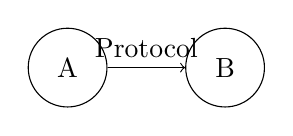
\begin{tikzpicture}
        \node[draw,circle,minimum size=1cm] (A) at (0,0) {A};
        \node[draw,circle,minimum size=1cm] (B) at (2,0) {B};
        \draw[->] (A) -- (B) node[midway,above] {Protocol};
    \end{tikzpicture}
    \caption{Simple protocol diagram}
    \label{fig:protocol}
\end{figure}

\subsection{Enhanced Captions}

The \texttt{captions} option provides improved caption formatting:

\begin{table}[h]
    \centering
    \begin{tabular}{lcc}
        \toprule
        Algorithm & Security Level & Key Size  \\
        \midrule
        AES-128   & 128 bits       & 128 bits  \\
        AES-256   & 256 bits       & 256 bits  \\
        RSA-2048  & 112 bits       & 2048 bits \\
        \bottomrule
    \end{tabular}
    \caption{Cryptographic algorithms comparison}
    \label{tab:algorithms}
\end{table}

\subsection{Cryptography Macros}

The \texttt{crypto} option provides specialized macros for cryptographic
notation:

\begin{itemize}
    \item $\mathcal{K}$ - Key space
    \item $\mathcal{M}$ - Message space
    \item $\mathcal{C}$ - Ciphertext space
    \item $\mathsf{Gen}$ - Key generation algorithm
    \item $\mathsf{Enc}$ - Encryption algorithm
    \item $\mathsf{Dec}$ - Decryption algorithm
\end{itemize}

\section{Usage Examples}

\subsection{Basic Usage}

For basic usage with minimal features:

\begin{verbatim}
\documentclass{llncs}
\usepackage{llncscrypto}
\end{verbatim}

\subsection{Full Feature Set}

For all features:

\begin{verbatim}
\documentclass{llncs}
\usepackage[captions,tikz,appendix,crypto,theorems]{llncscrypto}
\end{verbatim}

\subsection{Selective Features}

For specific features only:

\begin{verbatim}
\documentclass{llncs}
\usepackage[tikz,theorems]{llncscrypto}
\end{verbatim}

\section{Advanced Features}

\subsection{Cross-Referencing}

The package provides enhanced cross-referencing capabilities. For example, we
can reference Theorem~\ref{thm:security}, Definition~\ref{def:primitive}, and
Figure~\ref{fig:protocol}.

\subsection{Appendix Support}

The \texttt{appendix} option enables enhanced appendix management:

\begin{verbatim}
\appendix
\section{Additional Proofs}
\end{verbatim}

\section{Compatibility}

The \textsf{llncscrypto} package is designed to be fully compatible with:
\begin{itemize}
    \item LNCS document class
    \item Standard LaTeX packages
    \item pdfLaTeX, XeLaTeX, and LuaLaTeX engines
    \item Major TeX distributions
\end{itemize}

\section{Conclusion}

The \textsf{llncscrypto} package provides a comprehensive solution for
enhancing LNCS documents with advanced features for cryptography and
theoretical computer science research. It maintains compatibility with LNCS
requirements while adding powerful tools for modern academic writing.

\bibliographystyle{splncs04}
\begin{thebibliography}{8}

    \bibitem{ref1}
    Author, A.: Title of the paper. In: Proceedings of the Conference, pp. 1--10 (2023)

    \bibitem{ref2}
    Author, B., Author, C.: Another important paper. Journal of Cryptography 15(2), 123--145 (2024)

\end{thebibliography}

\end{document}